\chapter{Results}
The group ended up with a computer that managed to produce vector graphics according to design.
This chapter presents the results of the project.
The physical result is depicted in Figure \ref{fig:board-top}.
The advanced tunnel program that was produced (see Appendix \ref{app:tunnel}), can be seen in action here: \href{https://vid.me/JEZv}{https://vid.me/JEZv} \cite{tunnel-demo}.

\begin{figure}[h!]
	    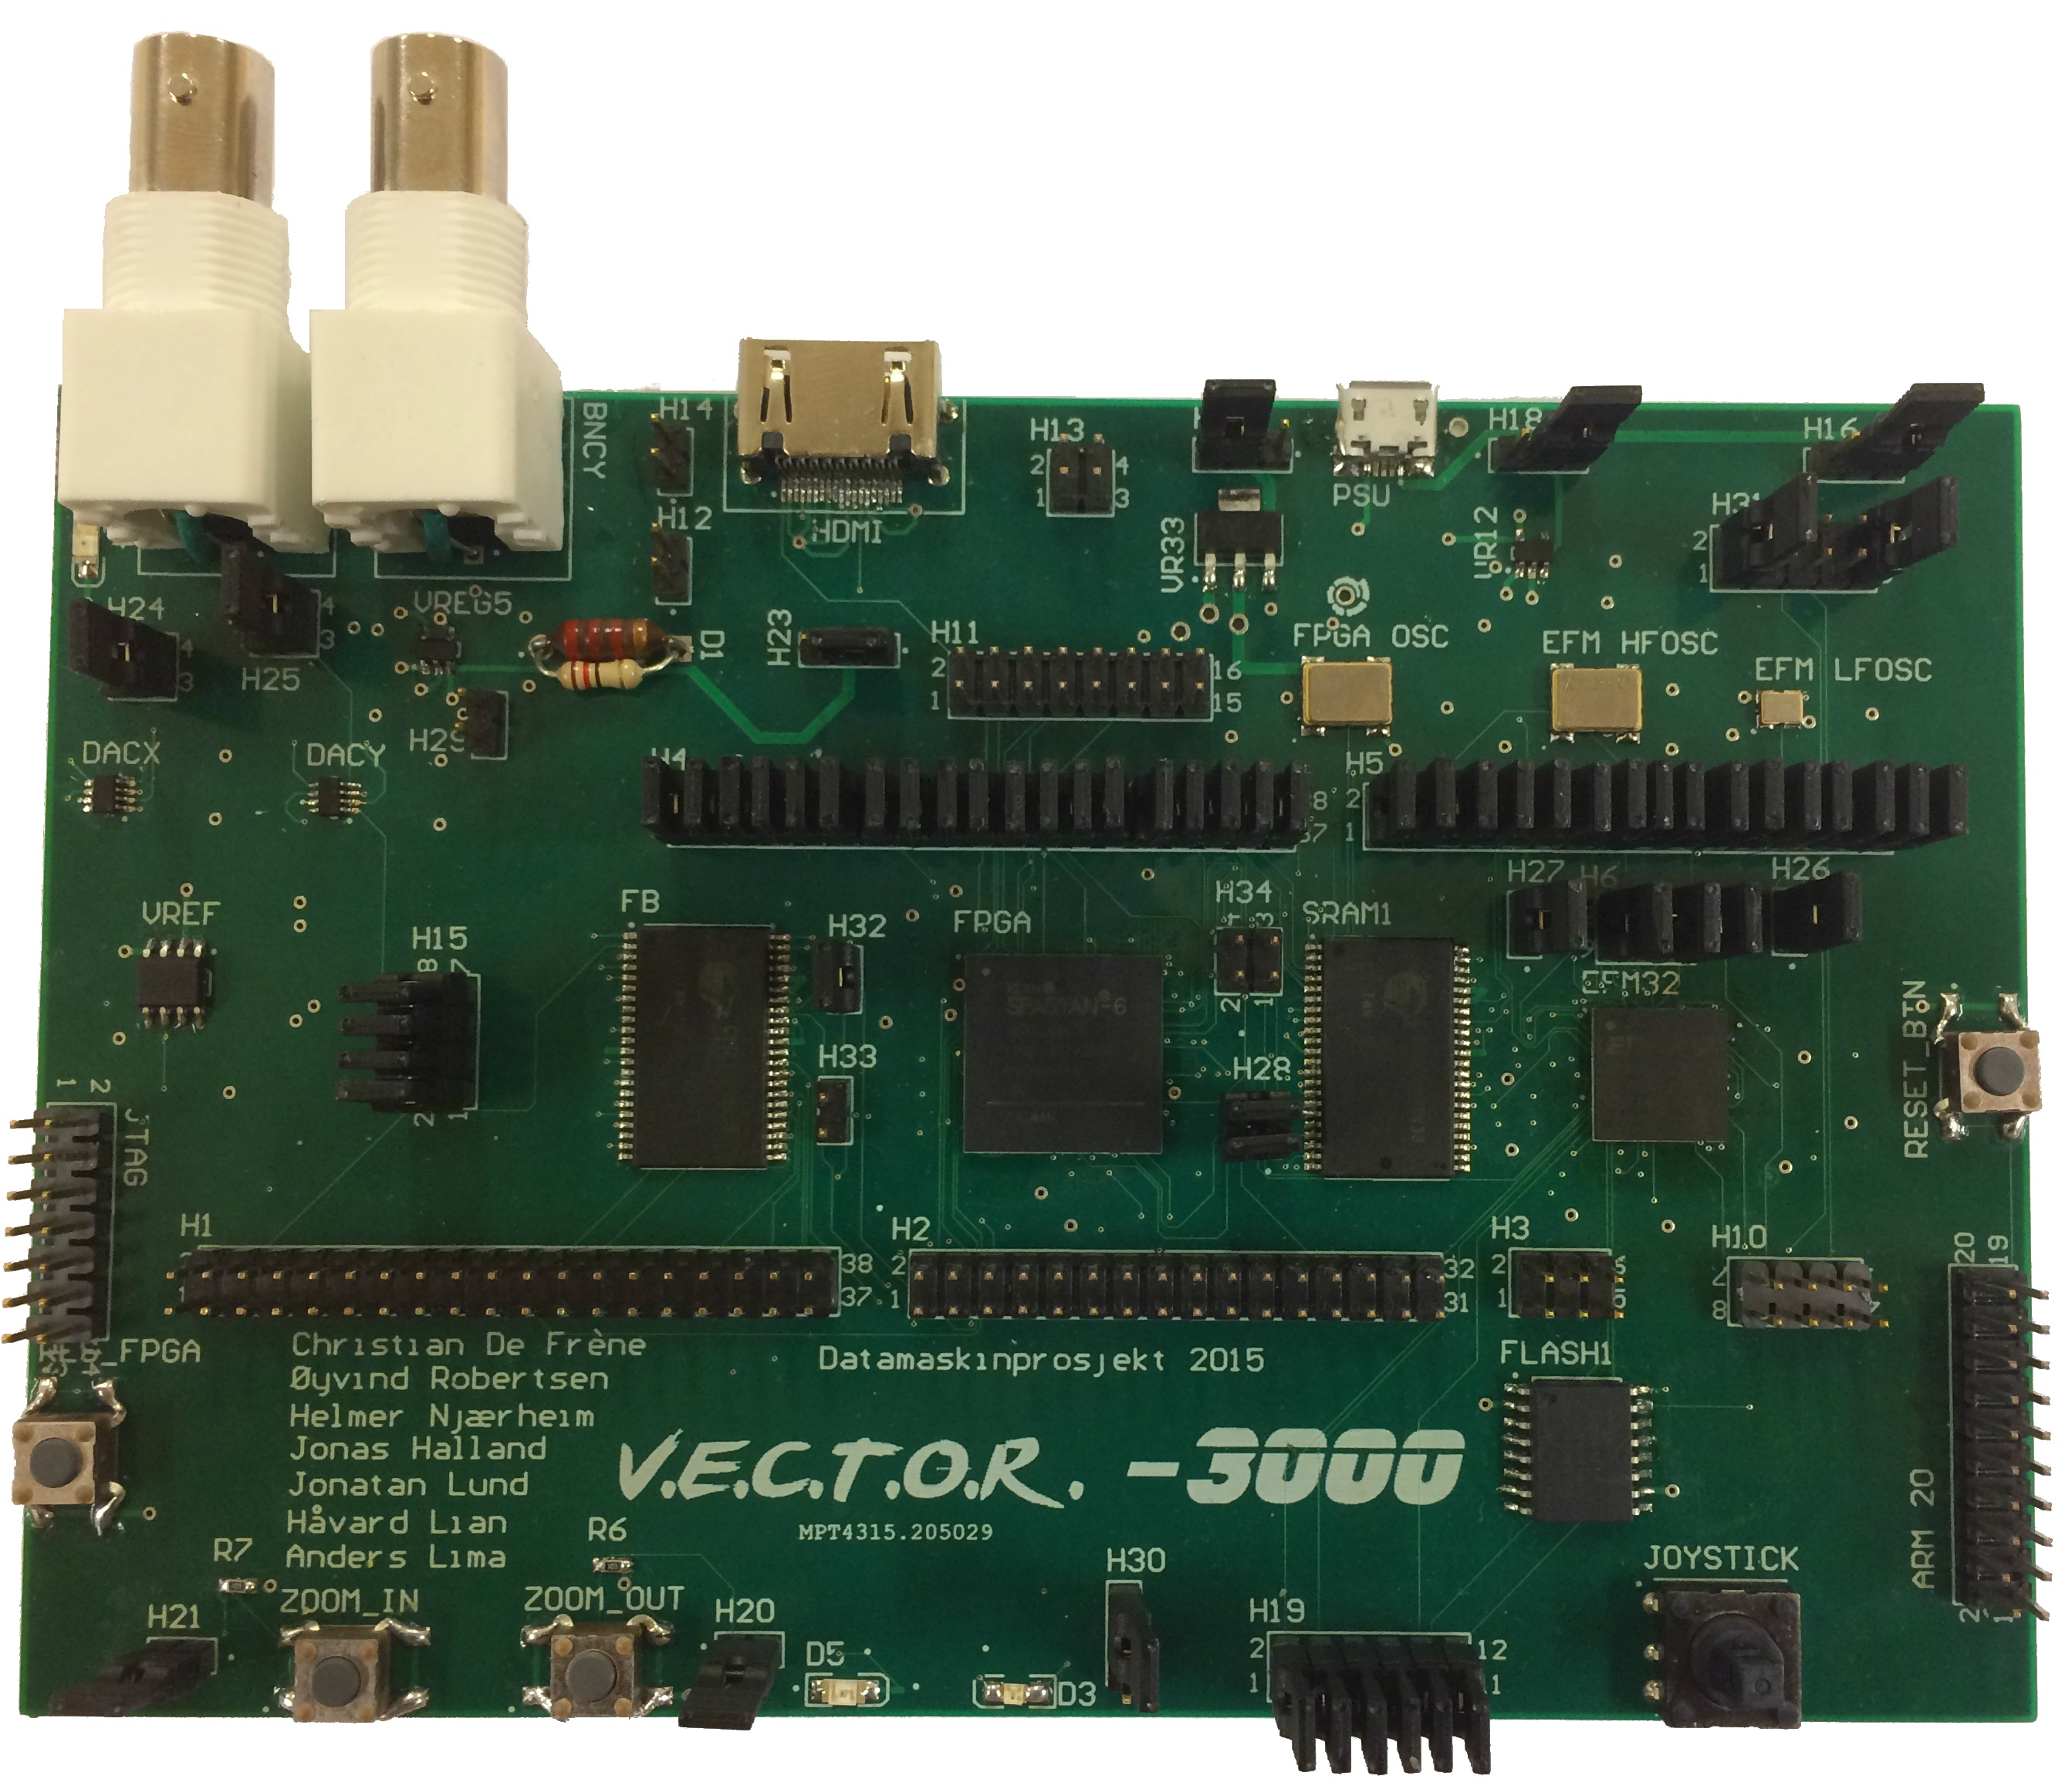
\includegraphics[width=\linewidth]{images/board_top.jpg}
	    \caption{An image of the finished \vthreek board}
	    \label{fig:board-top}
\end{figure}

\section{Memory}

The final implementation utilizes \gls{bram} not only to store the scene, but the instructions for the CPU as well.
This was done because the group was unable to get the SRAM chip that was on the three-way EBI bus to work properly.
Because of this the instructions for the CPU needs to be stored in the .bit file that programs the FPGA.

The SRAM chip dedicated to frame-buffer was also left unused as the group did not find the time to implement a raster output module.

\section{Performance}

The maximum clock frequency of the DACs is 30MHz according to the datasheet \cite{dac-datasheet}.
To update the DAC value a total of 25 clock cycles are required.
As a result the theoretical effective maximum output will be \(30 MHz \div 25 = 1.2 MHz \).
However during testing the group experience incorrect \gls{dac} values if the clock were set higher than 20 MHz.
With a clock frequency of 20 MHz the maximum output is 800 KHz.

The CPU can be clocked significantly faster than it is in the current design, but since the output module needs to be run at 20 MHz this was chosen for the CPU as well for simplicity.
At 20 MHz the CPU is still more than fast enough to update primitives in order to achieve smooth animations, so busy loops was introduced in the primitive update procedures in order to slow the update rate down.

\section{Noise}

As the main output is analogue it is susceptible to electronic noise. This noise represents itself as unwanted changes in voltage. 
The system was design to have as little noise as possible, and under operation the mean noise on the signal is around 40mV.
A measure of this is shown in Figure~\ref{fig:noise}.

\begin{figure}[H]
	    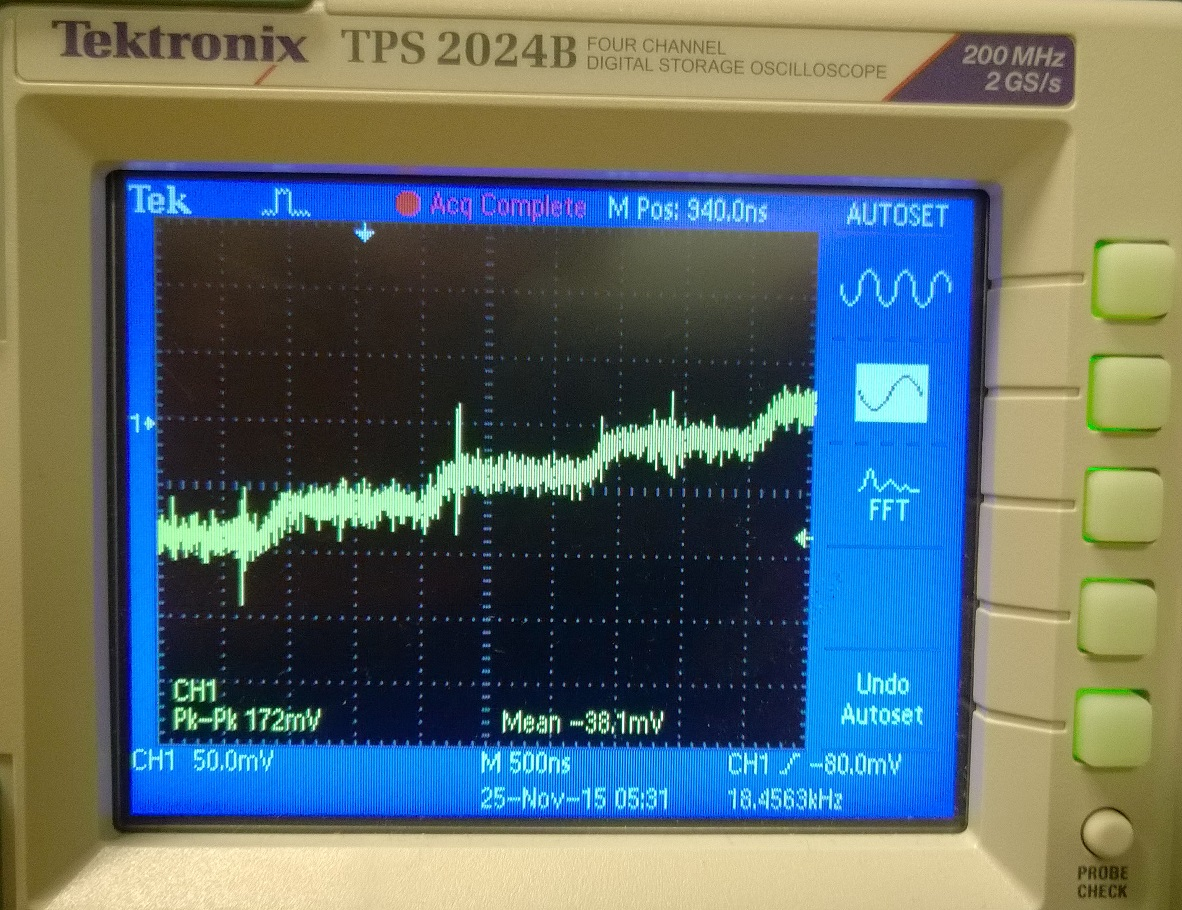
\includegraphics[width=\linewidth]{images/noise}
	    \caption{The noise on the voltages from the DACs}
	    \label{fig:noise}
\end{figure}



\section{Video Output}
\vthreek was successful in drawing primitives to a screen.
Only one of the output modules, the analogue oscilloscope output, were realized.
This section presents the results from this module.

\subsection{Oscilloscope}
In Figure \ref{fig:square}, one can see great improvement in the accuracy when drawing a square, compared to the result in Figure \ref{fig:osc_poc}.

\begin{figure}[h!]
	    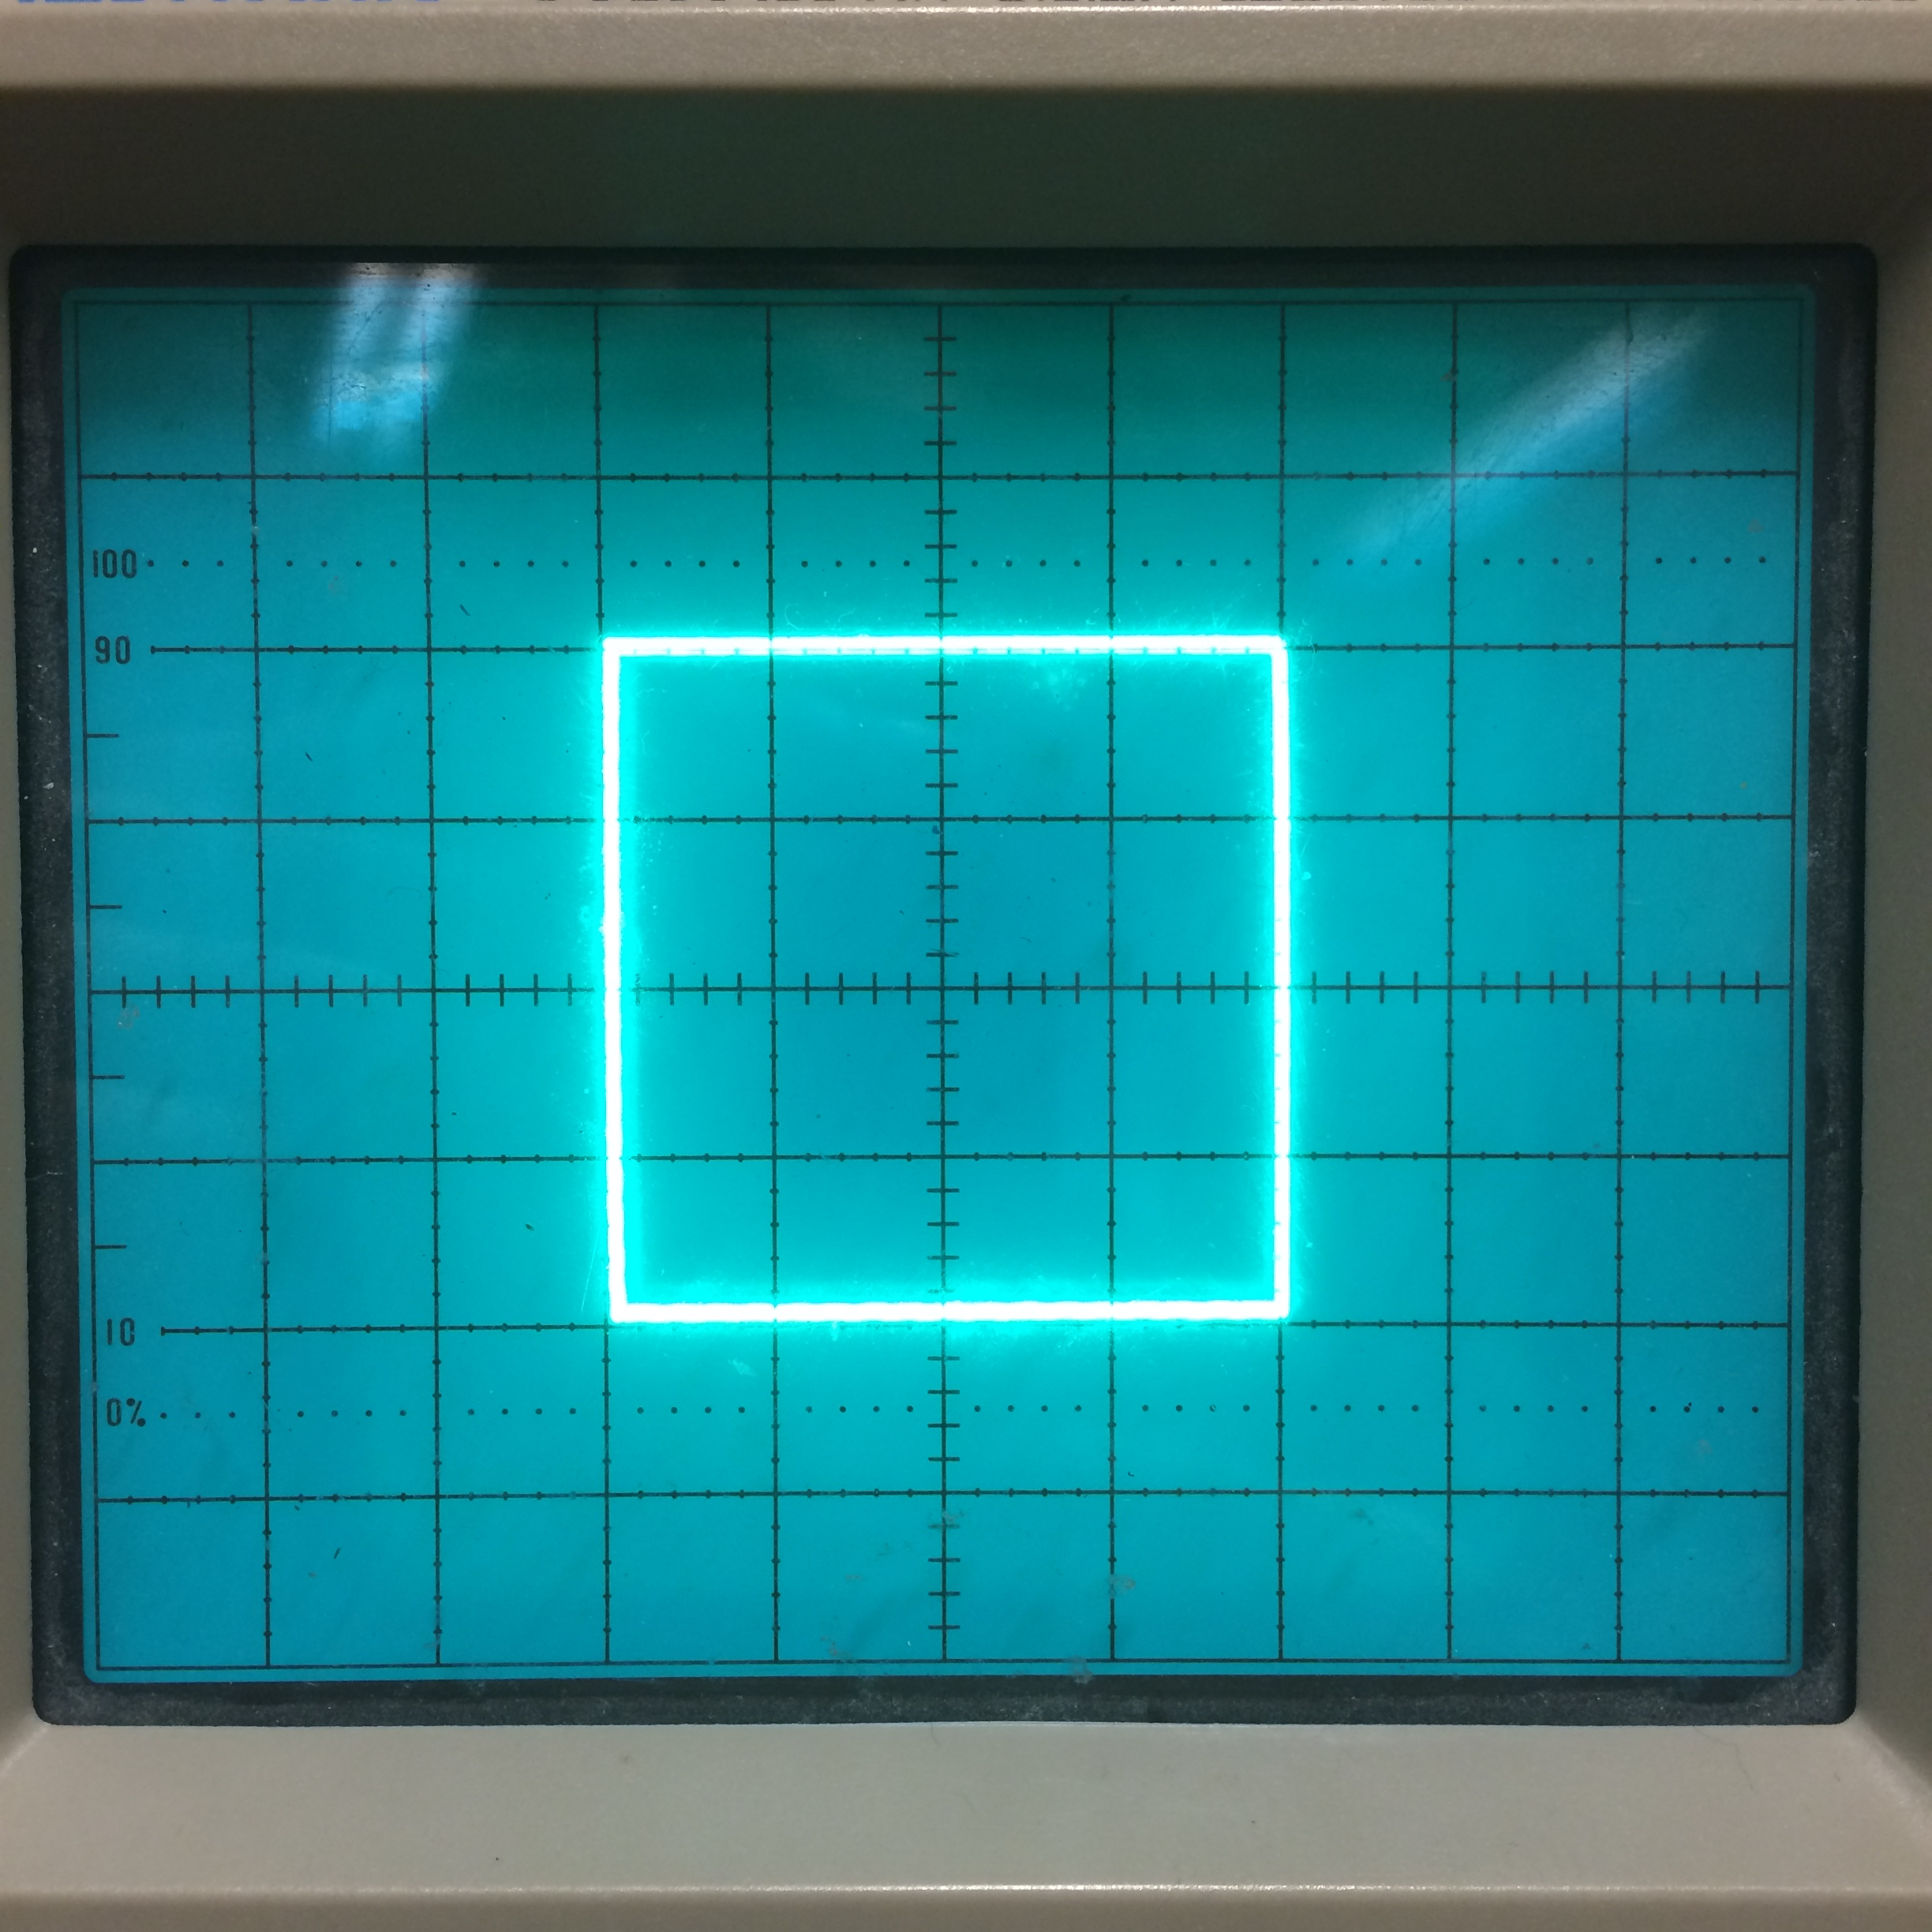
\includegraphics[width=\linewidth]{images/square}
	    \caption{A square drawn with the finished implementation}
	    \label{fig:square}
\end{figure}


\subsubsection{Drawing Artefacts}
\label{results:artefacts}
Even though drawing to the oscilloscope looks nice, some artefacts were discovered.
When the oscilloscope is done drawing one primitive and moves to the next the electron beam is still drawing,
and weaker drawing lines may be visible.
In other words all shapes are drawn without "lifting the pencil off the paper".
If one take a closer look at Figure \ref{fig:artefact}, the drawing artefacts are visible.
There are solutions to avoid the drawing artefacts, which is explained in Section \ref{discussion:artefacts}.

\begin{figure}[h!]
	    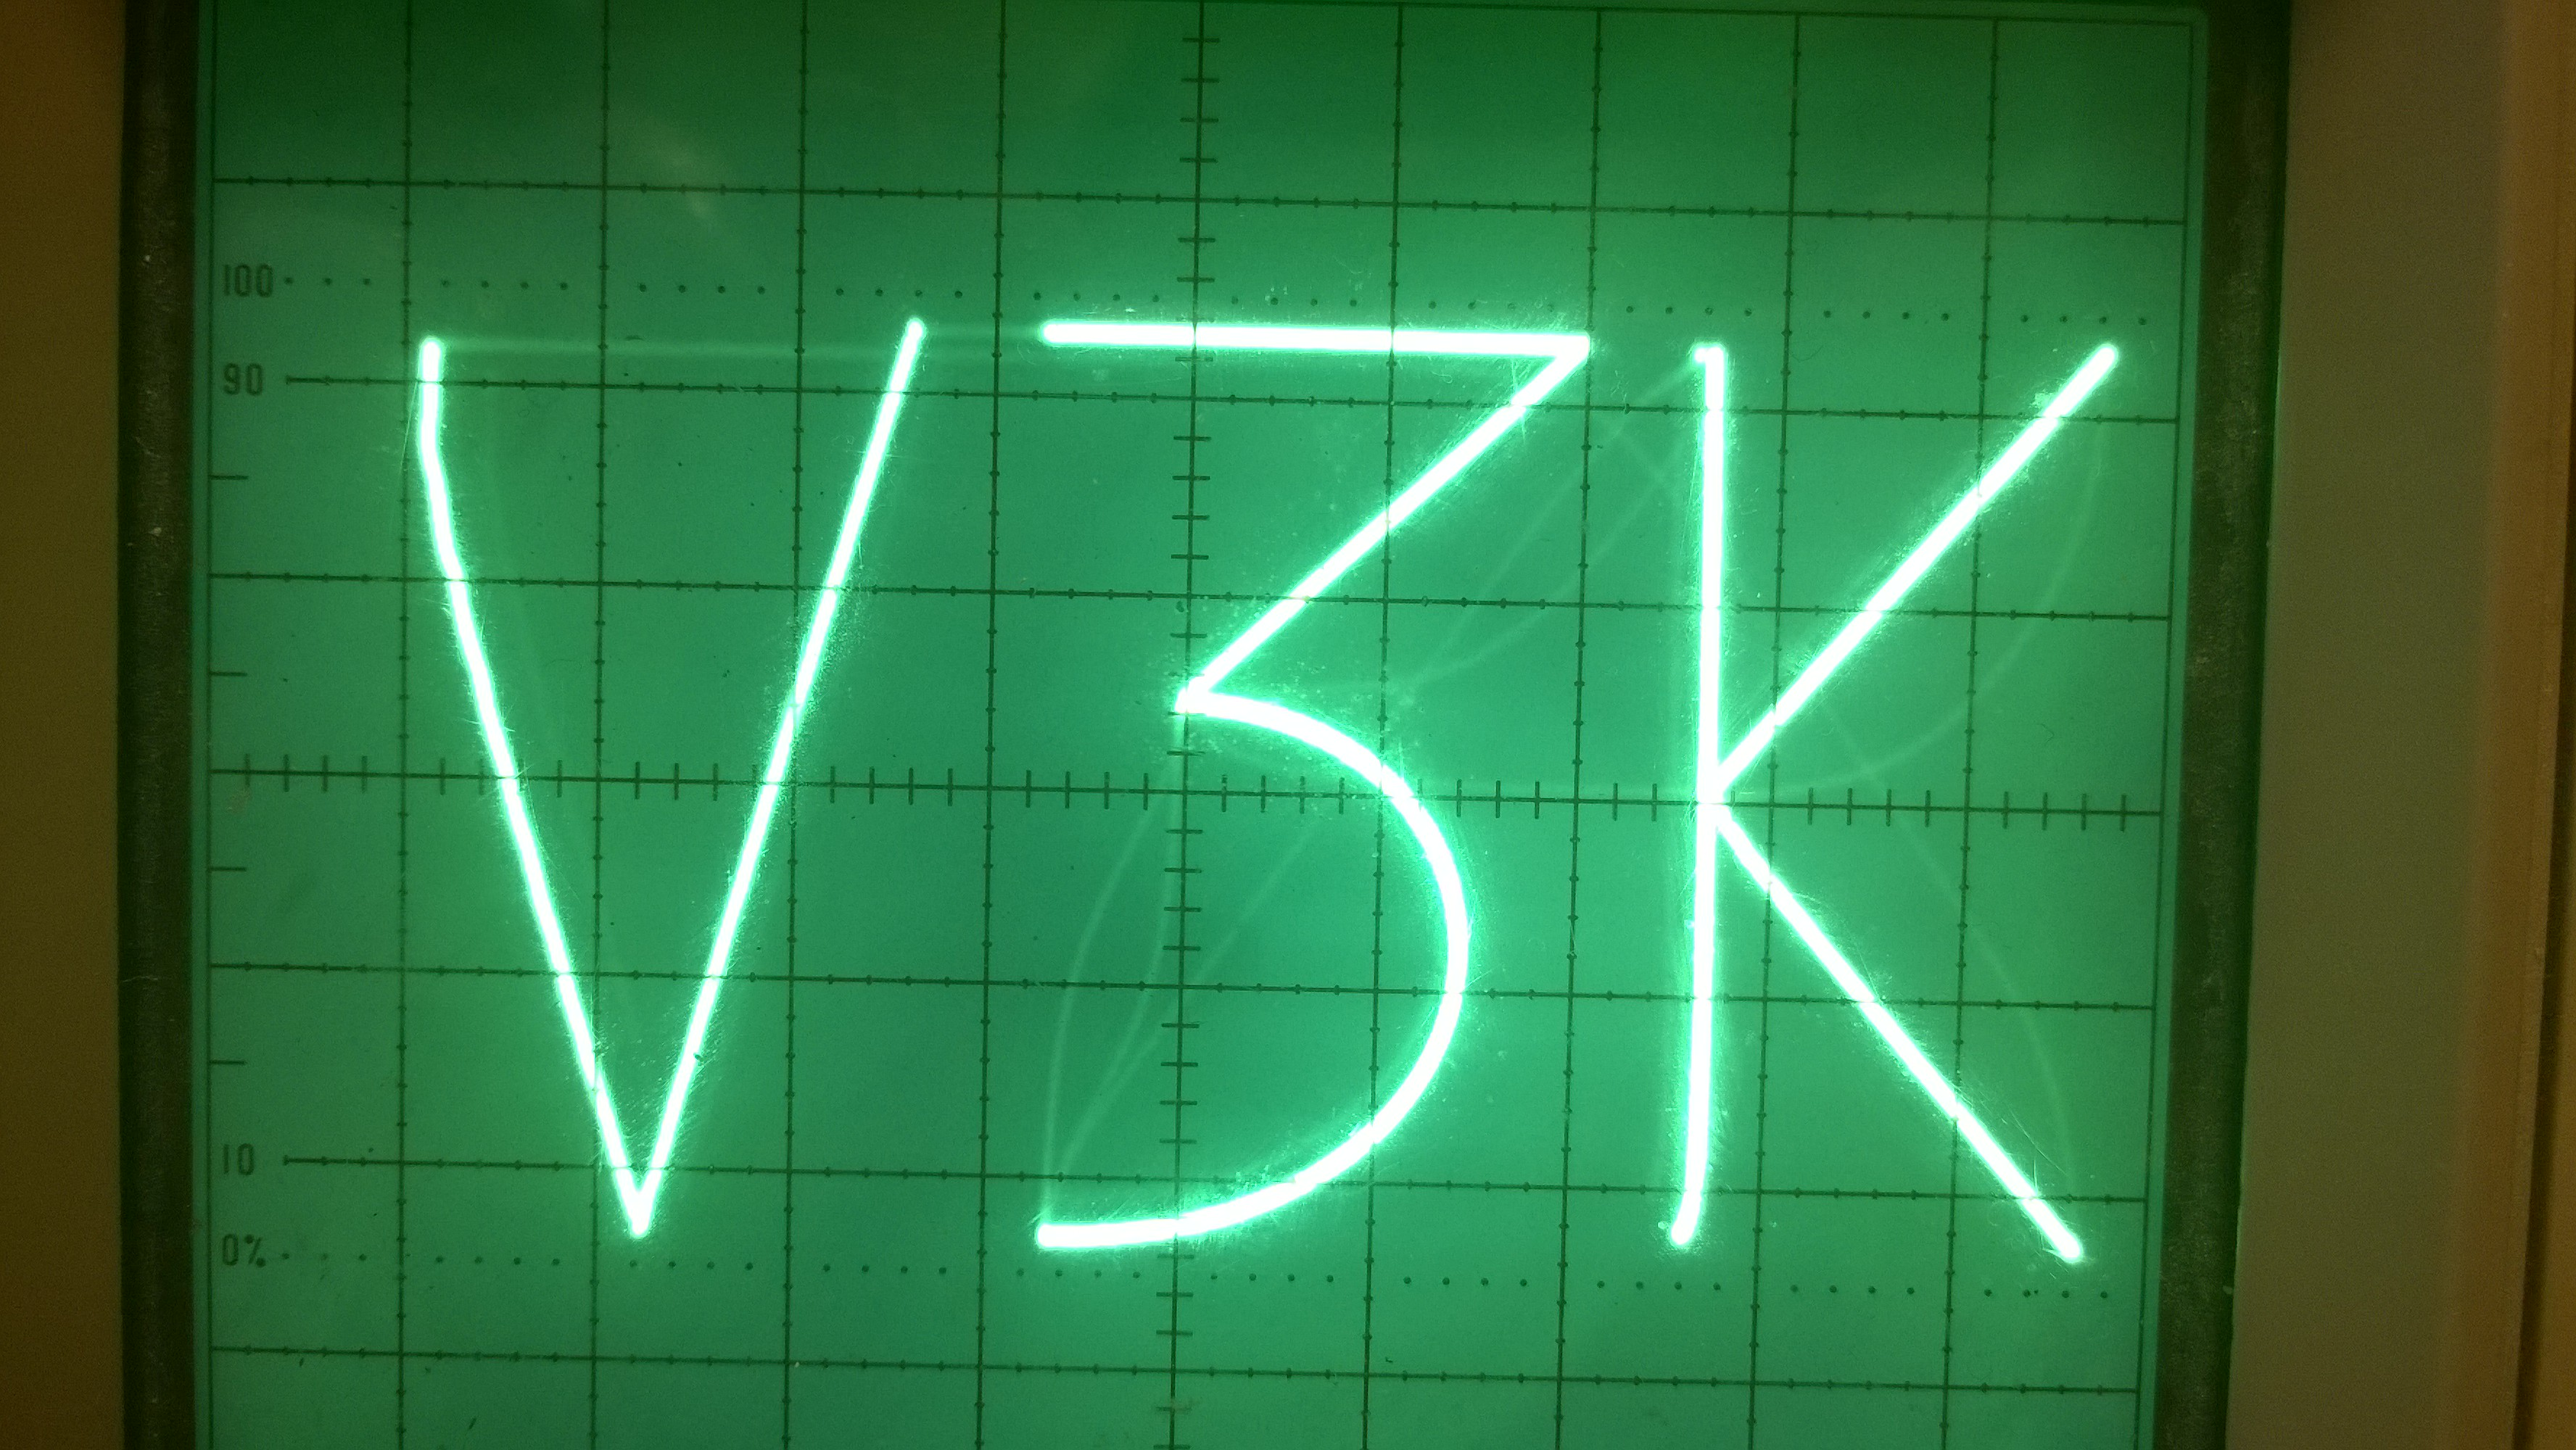
\includegraphics[width=\linewidth]{images/artefacts.jpg}
	    \caption{Drawing V3K with artefacts}
	    \label{fig:artefact}
\end{figure}

Another artefact, also barely visible, is the dots that each primitive is made of.
By zooming in on the oscilloscope this becomes more visible, and can be seen in Figure \ref{fig:artefact-dots}.
The digital nature of \vthreek results in discrete increments when drawing.
The electron ray moves faster than the \gls{dac}s are able to feed it with new data.
As a result, the ray will wait at one spot, until it receives new values.
This results in dotted lines, shown in Figure \ref{fig:dotx4} and \ref{fig:dotx8}

\begin{figure}[h!]
   	\centering
    \begin{subfigure}[b]{\textwidth}
   		\centering
       	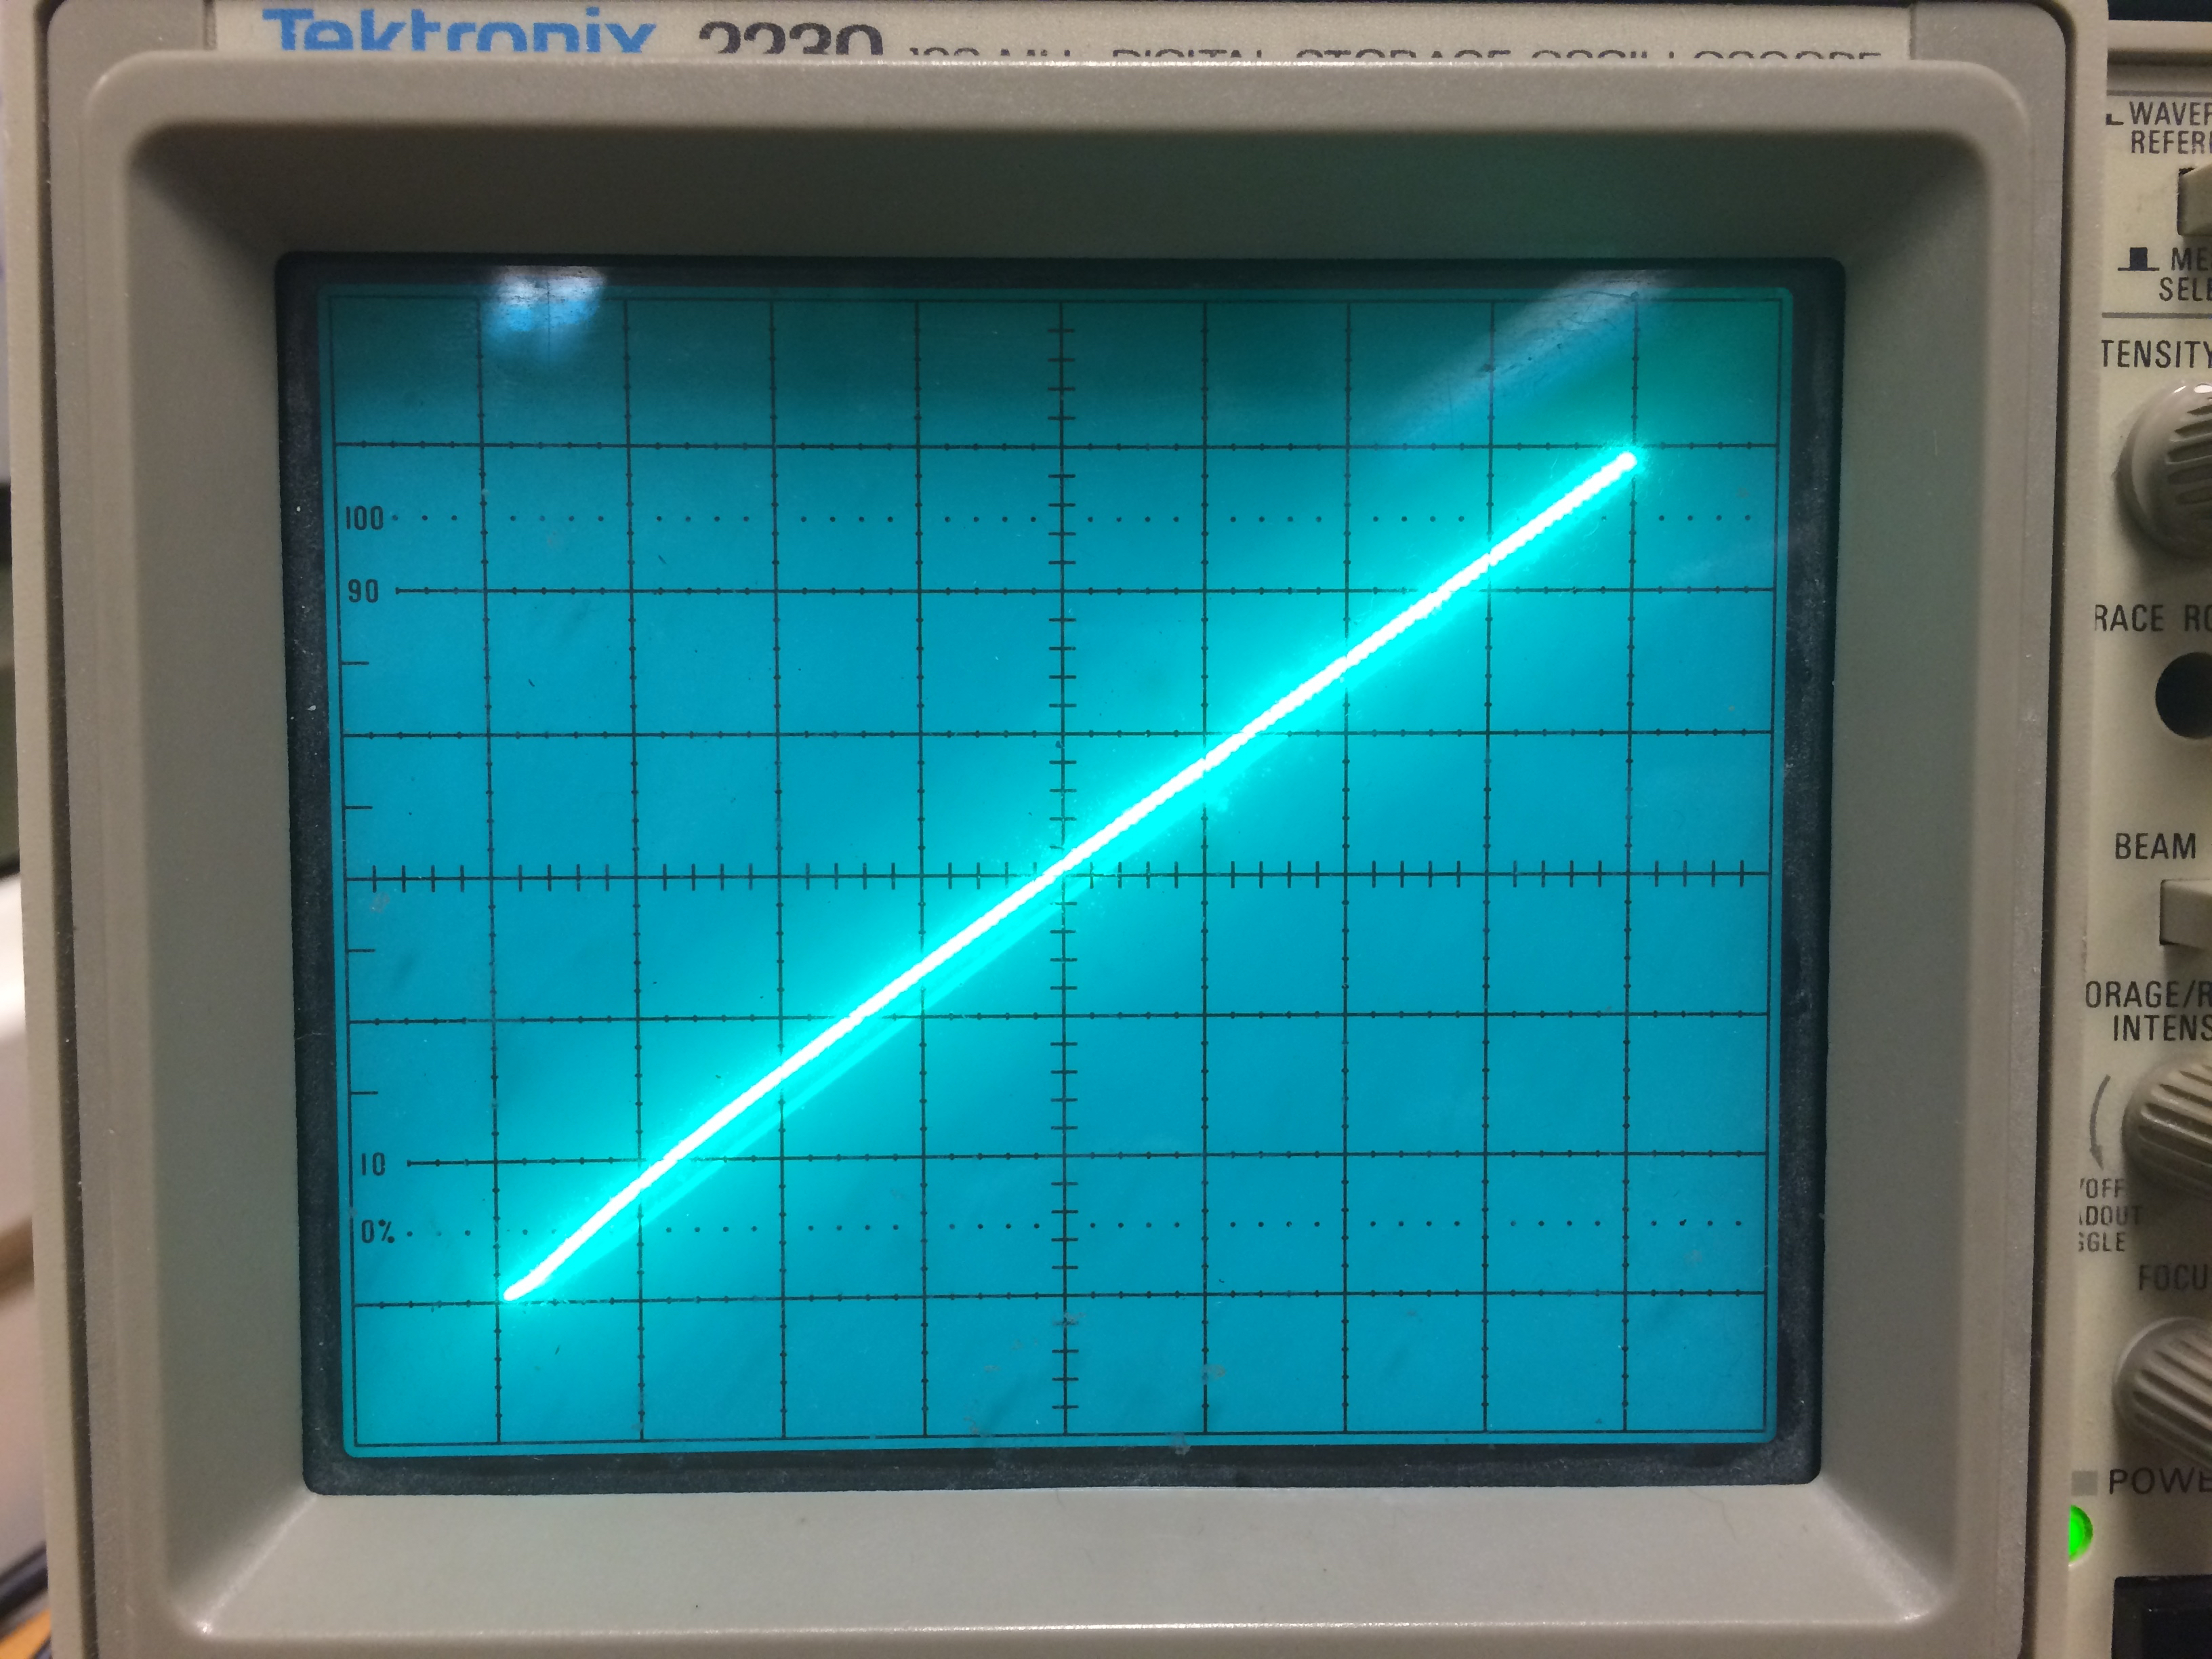
\includegraphics[height=0.4\textheight]{images/dots_x1.jpg}
       	\caption{Dot artefact close to invisible.}
       	\label{fig:dotx1}
    \end{subfigure}
\end{figure}

\begin{figure}[h!]
	\ContinuedFloat
    \begin{subfigure}[b]{\textwidth}
		\centering
        \includegraphics[height=0.4\textheight]{images/dots_x4.jpg}
        \caption{Dot artefact becomes more visible when zoomed in four times.}
        \label{fig:dotx4}
    \end{subfigure}

    \begin{subfigure}[b]{\textwidth}
		\centering
        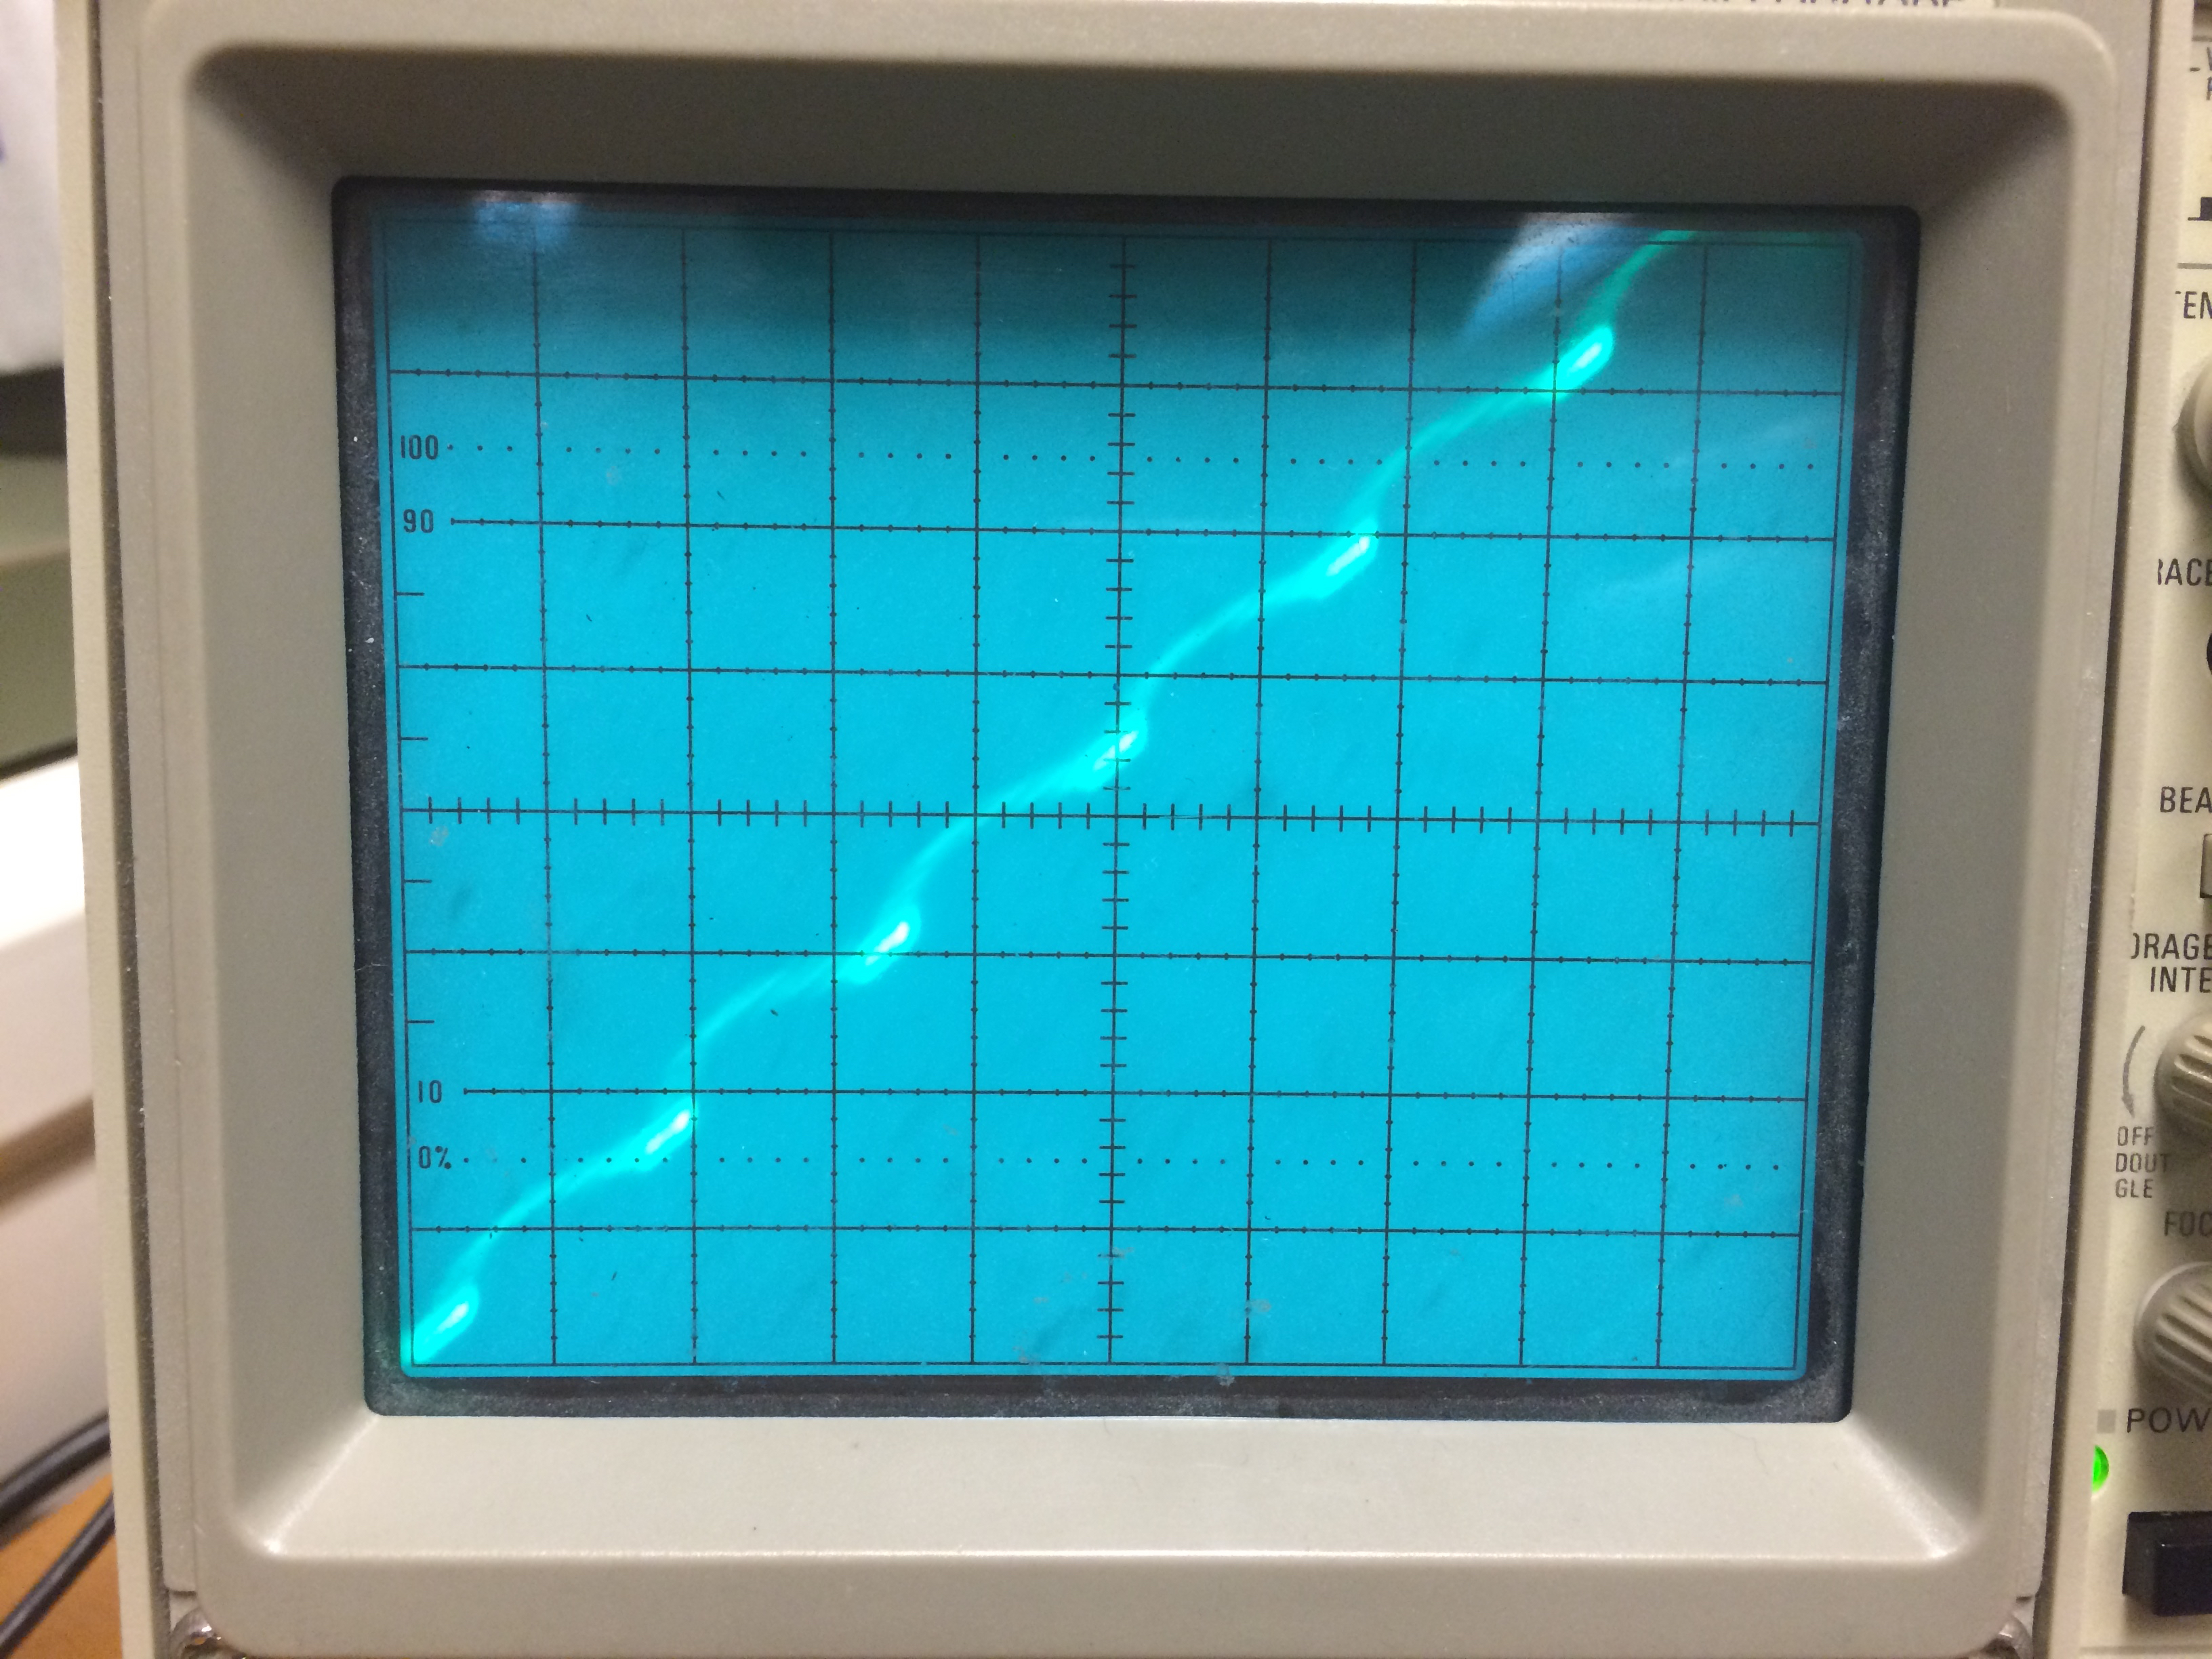
\includegraphics[height=0.4\textheight]{images/dots_x8.jpg}
        \caption{Zooming in eight times, it can be observed that the electron ray do not move in a straight line from point to point.}
        \label{fig:dotx8}
    \end{subfigure}
    \caption{A diagonal line with different levels of zoom}
    \label{fig:artefact-dots}
\end{figure}

\subsection{HDMI}
Rasterisation and \gls{hdmi} were not implemented.
The intention of this part was to demonstrate the difference between vector and raster output in real-time.
However, these parts of the system were no longer prioritized when the analogue counterpart proved to be a reliable source of output.
Moreover, this part was a medium priority requirement, listed in Table \ref{tbl:non_func_req}, and thus not a critical part of \vthreek.

\section{Budget}
In the assignment text, the group was given a budget of 10,000 NOK.
At the end of the project the total cost of materials was about 11,500 NOK (without shipping costs), which is somewhat above the proposed budget for the project.
The full list of material expenses is listed in Appendix \ref{tbl:material-cost}.
